\documentclass[main]{subfiles}

\begin{document}
\begin{lect}{2019-10-03}
		\begin{Reminder}
				\[M(x, y)dx + N(x,y)dy = 0 \q(1) \qq M, N \in C(G)\]
				\[y = \varphi(x) \text{ - реш (1), } x \in (a, b) \rla \]
				\[\rla M(x, \varphi(x)) + N(x, \varphi(x)) \varphi'(x) \equiv 0 \text{ на } (a, b)\]
		\end{Reminder}

		\begin{Definition}
				\[u(x, y) \in C^{1}(G)\]
				Интл (1), если
				\begin{enumerate}
						\item хоть одна из $\frac{\partial u}{\partial x}, \frac{\partial u}{\partial y}$ не 0 в $\forall $
							обыкн. точке $G$
						\item $N \cdot \frac{\partial u}{\partial x} - M \frac{\partial u}{\partial y} \equiv 0$ в $G \qq (4)$
				\end{enumerate}
		\end{Definition}

		\[(5) \qq u(x, y) = u(x_0, y_0) \qq (x_0, y_0) \in G\]
		\[u \text{ - инт-л (1) в } G\]
		\begin{Theorem} [2]
				\[N(x_0, y_0) \neq 0 \Ra\]
				рав-во (5) разрешимо отн $y$: его решение
				\[y = \varphi(x) \text{ опред на }(a, b) \q x_0 \in (a, b) \q \varphi(x_0) = y_0\]
				\[y = \varphi(x) \text{ непр дифф на } (a, b) \text{ и явля реш ур } (1)\]
		\end{Theorem}

		\begin{Proof}
				\[N(x_0, y_0) \neq 0 \Ra N(x, y) \neq 0 \text{ в нек. окр-ти } V(x_0, y_0)\]
				\[\Ra \frac{\partial u(x_0, y_0)}{\partial y} \neq 0 (\text{ из (4): если } \frac{\partial u(x_0, y_0)}
				{\partial y} = 0 \text{, то } \frac{\partial u(x_0, y_0)}{\partial x} = 0)\]
				Противореч. с тем, что $(x_0, y_0)$ - обыкн
				\[\Ra \frac{\partial u(x, y)}{\partial y} \neq 0 \text{ в нек. окр } \widetilde{V}(x_0, y_0)\]
				\[\Ra \text{ теорема о неявн. функции} \q \exists  y = \varphi(x) \text{ - реш } (5) : y_0 = \varphi(x_0)\]
				\[\varphi(x) \text{ - непр дифф} \qq x \in (a, b) \q (x_0 \in (a, b))\]
				\[u(x, \varphi(x)) = u(x_0, y_0) \text{ на } (a, b)\]
				\[\frac{\partial u}{\partial x} + \frac{\partial u}{\partial y} \cdot \varphi'(x) = 0 \Ra
				\varphi'(x) = - \frac{\frac{\partial u(x, \varphi(x))}{\partial x}}{\frac{\partial u(x, \varphi(x))}
				{\partial y}}\]
				\[\text{в (2) } M(...) + N(...) \left(-\frac{\frac{\partial u(...)}{\partial x}}
				{\frac{\partial u}{\partial y}(...)}\right) = \]
				\[ = -\frac{1}{\frac{\partial u}{\partial y}(...)} [N(...)\frac{\partial u}{\partial x}(...) -
				M(...) \frac{\partial u(...)}{\partial y}] \equiv 0 \text{ в }G\]
		\end{Proof}

		\begin{Theorem} [2]

		\end{Theorem}

		\begin{Consequence}
				\[(x_0, y_0) \text{ - обыкн точка } G \text{, то рав-во (5)} \]
				разреши. отн $y$ или отн $x$ и его реш - реш (1)
				\[(M \neq 0 \text{ или } N \neq 0)\]
		\end{Consequence}

		\begin{definition}
				равн-во $u(x, y) = c$ - общ. инт-л (1)
		\end{definition}

		\begin{Example}
				\[xdx + ydy = 0\]
				\[\underbrace{x^2 + y^2}_{u(x, y)}  = c\]
				\begin{figure}[H]
						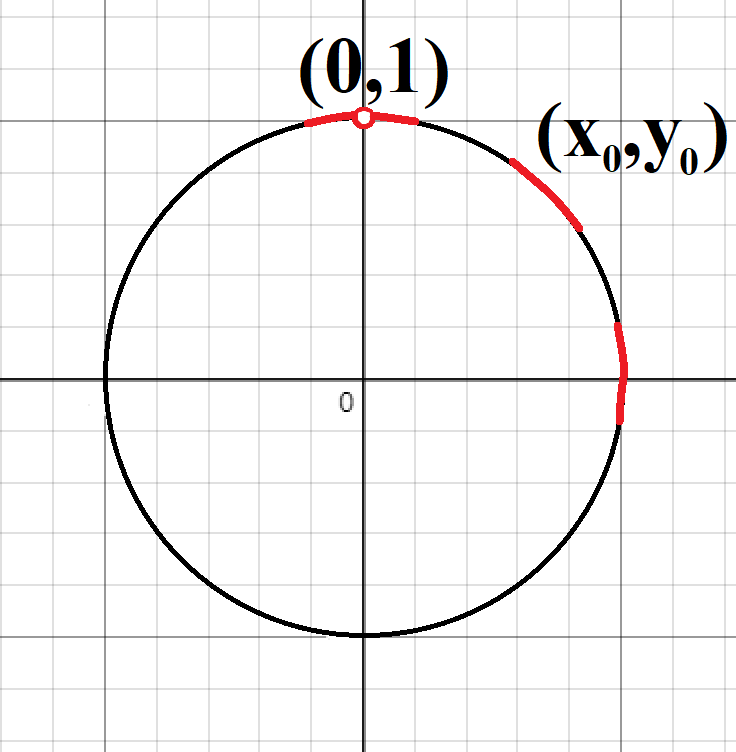
\includegraphics[width=4cm]{pics/5_1.png}
						\centering
				\end{figure}
		\end{Example}

		\section{Уравнения в полных дифф.}

		\[M(x, y)dx + N(x, y)dy = 0 \qq (1)\]

		\begin{definition}
				(1) - ур в полных дифф, если
				\[\exists u(x, y) : \q du(x, y) = M(x, y)dx + N(x, y)dy \qq (2)\]
				\[( (1) : du = 0) \]
		\end{definition}

		\begin{theorem}[1]
				(1) - ур в полных дифф $\Ra$ $u(x, y)$ - инт-л (1)
		\end{theorem}

		\begin{proof}
		    \begin{enumerate}
						\item $u(x, y)$ - непр дифф.
						\item $\displaystyle  \frac{\partial u}{\partial x} = M, \q \frac{\partial u}{\partial y} = N \qq (3)$
						\item $N \frac{\partial u}{\partial x} - M \frac{\partial u}{\partial y} = N \cdot M - M \cdot N \equiv 0$
		    \end{enumerate}
		\end{proof}

		\begin{Theorem}
				\[\text{если } \exists  \frac{\partial M}{\partial y}, \frac{\partial N}{\partial x} \in C(G) \q
				(1) \text{ - ур. в полных дифф}\]
				\[\text{то } \frac{\partial M}{\partial y} = \frac{\partial N}{\partial x} \text{ в } G \qq (4)\]
		\end{Theorem}

		\begin{Proof}
				\[(1) \text{ - ур в п. дифф} \Ra \exists u(x, y) \q (2), (3)\]
				\[\Ra \frac{\partial M}{\partial y} = \frac{\partial ^2 u}{\partial y \partial x} \ = \
				\frac{\partial^2 u}{\partial x \partial y} = \frac{\partial N}{\partial x}\]
		\end{Proof}

		\[G = \{(x, y) : \ a < x < b, c < y < d\}\]
		\[(\text{м.б } a = -\infty,\ c = -\infty \qq b = +\infty,\ d = +\infty)\]

		\begin{Theorem} [3]
				\[\exists \frac{\partial M}{\partial y}, \frac{\partial N}{\partial x} \in C(G)\]
				\[\text{И вып } (4) \Ra (1) \text{ - ур. в п. д.}\]
		\end{Theorem}

		\begin{Proof}
				\[(x_0, y_0), (x, y) \in G\]
				\begin{figure}[H]
						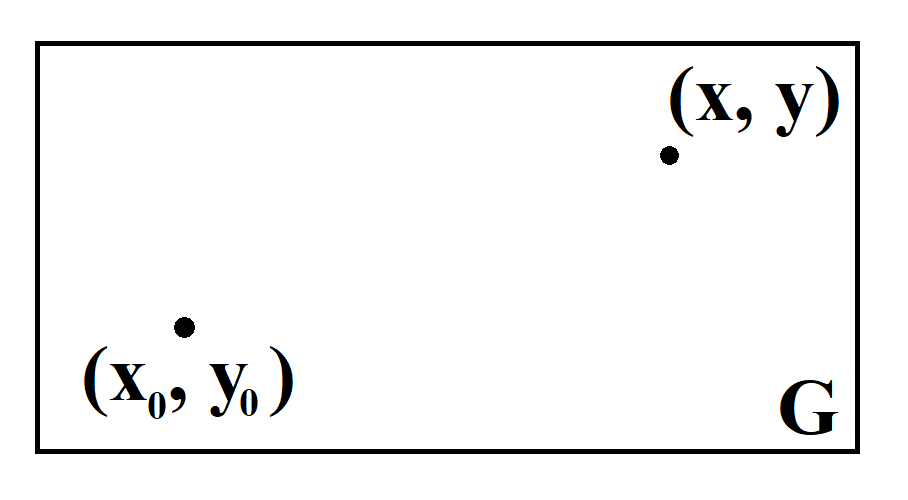
\includegraphics[width=4cm]{pics/5_2.png}
						\centering
				\end{figure}
				\[\forall t \in [x_0, x] \q (t, y) \in G\]
				\[\frac{\partial u(t, y)}{\partial x} = M(t, y) \text{ - инт от } x_0 \text{ до } x\]
				\[u(x, y) - u(x_0, y) = \int_{x_0}^x M(t, y)dt \qq (5)\]
				\[\forall t \in [y_0, y] \q (x_0, y) \in G\]
				\[\frac{\partial u(x_0, t)}{\partial y} = N(x_0, t) \text{ - инт от } y_0 \text{ до } y\]
				\[u(x_0, y) - \underbrace{u(x_0, y_0)}_{\text{НУО } = 0}  = \int_{y_0}^y N(x_0, t) dt \qq (6) \]
				\[u(x,y) = \int_{x_0}^x M(t, y)dt + \int_{y_0}^y N(x_0, t)dt  \qq (7)\]
				Проверяем, что это та функция, которая нужна
				\[\frac{\partial u(x, y)}{\partial x} = M(x, y)\]
				\[\frac{\partial u(x, y)}{\partial y} = \frac{\partial }{\partial y} \int_{x_0}^x M(t, y)dt + N(x_0, y) =
				\int_{x_0}^x \frac{\partial M(t, y)}{\partial y}dt + N(x_0, y) =  \]
				\[ = \int_{x_0}^x \frac{\partial N(t, y)}{\partial t}dt + N(x_0, y) =
				N(x, y) - N(x_0, y) + N(x_0, y)\]
		\end{Proof}

		\begin{Remark} [1]
				\[u(x, y) = \int_{x_0}^x M(t, y_0)dt + \int_{y_0}^y N(x, t)dt  \qq (7')\]
				\begin{figure}[H]
						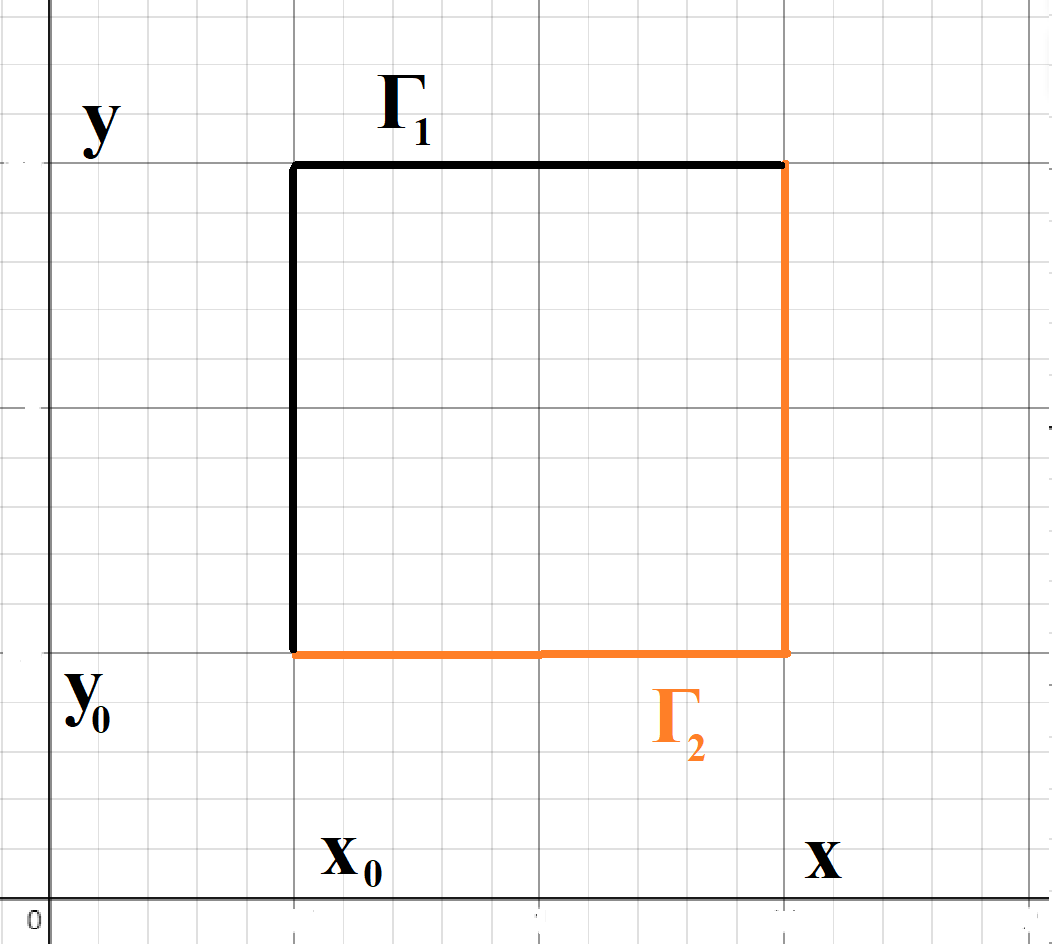
\includegraphics[width=4cm]{pics/5_3.png}
						\centering
				\end{figure}
		\end{Remark}

		\begin{Utv}
				\[du(x, y) = M(x,y)dx + N(x, y)dy \q \text{Вып (4)} \q G \text{ - односвяз.}\]
				\[\Ra u(x, y) = \int_{\Gamma} M(x,y)dx + N(x,y)dy \qq (8) \text{ - криволин. инт}\]
				\[\Gamma \text{ - любая кривая, соед } (x_0, y_0), (x, y)\]
				Условие (4) гарантирует нам, что криволин. интеграл не зависит от кривой интегрирования
		\end{Utv}

		\begin{remark} [2]
				Прямоугольность области $G$ не требуется по-существу, нужна только односвязность (отсутсвие дырок или возможность стянуть любой путь в точку)
		\end{remark}

		\begin{Definition}
				\[(1) \qq \mu = \mu(x, y) \in C(G)  \qq \mu(x, y) \neq 0 \q \forall (x, y) \in G\]
				$\mu$ - интегр мн-ль для (1), если
				\[(9) \q (\mu M)dx + (\mu N)dy = 0 \text{ - ур. в п. д}\]

				\[\letus M, N, \mu \in C^1(G) \q (G \text{ - односвяз})\]
				\[(9) \text{ - ур в п.д.} \rla \frac{\partial }{\partial y}(\mu M) = \frac{\partial }{\partial x}(\mu N)\]
				\[\frac{\partial \mu}{\partial y}M + \mu \frac{\partial M}{\partial y} =
				\frac{\partial \mu}{\partial x}N + \mu \frac{\partial N}{\partial x} \qq (1)\]
				Частный случай 1
				\[\underline{\mu = \mu(x)}\]
				\[\text{из (10):} \frac{d\mu}{dx}N = \mu (\frac{\partial M}{\partial y} -
				\frac{\partial N}{\partial x})\]
				\[\frac{1}{\mu} \cdot \frac{d\mu}{dx} = \frac{\frac{\partial M}{\partial y} - \frac{\partial N}{\partial x}}{N} \qq (11)\]
				\[N = f(x)\]
				\[\frac{d\mu}{\mu} = f(x)dx\]
				\[\mu = e^{\int f(x)dx} \]
				\[\mu(x) = e^{\int_{x_0}^x f(t)dt } \]
				Частный случай 2
				\[\underline{\mu = \mu(y)}\]
				\[\frac{1}{\mu} \frac{d\mu}{dy} = \frac{\frac{\partial N}{\partial x} - \frac{\partial M}{\partial y}}{M} \qq (12)\]
				\[M = g(y)\]
		\end{Definition}
\end{lect}
\end{document}
